\documentclass{zkdl-presentation-template}

% --- Bitcoin Script helpers ---
\usepackage{etoolbox}
\AtBeginEnvironment{tcolorbox}{\small}
\newtcolorbox{empheqboxed}{
  enhanced,
  boxsep=1pt,
  arc=0.75ex,
  colback=gray!10,
  colframe=gray!40,
  boxrule=1pt,
  leftrule=40pt,
  top=-3.5mm,
  overlay unbroken and first ={%
    \node[minimum width=1cm,
      anchor=south,
      font=\sffamily\bfseries,
      xshift=20pt,
      yshift=-6.5pt,
    black]
    at (frame.west) {\scriptsize Script:};
  }
}

\newcommand{\mycomment}[1]{}
\newcommand{\elem}[1]{\, \langle #1 \rangle \,}
\newcommand{\opcode}[1]{\, \texttt{#1} \,}
\newcommand{\script}[1]{ $\big\{ #1 \big\}$ }

% -- Algorithms --
\usepackage[
    titlenumbered,
    linesnumbered,
    ruled
]{algorithm2e}
\SetKwInOut{Input}{Input}
\SetKwInOut{Output}{Output}
\SetKwInOut{Return}{Return}

% --- Ticks and crosses ---
\usepackage{pifont} % http://ctan.org/pkg/pifont
\newcommand{\cmark}{\textcolor{green!65!black}{\ding{51}}}%
\newcommand{\xmark}{\textcolor{red!80!black}{\ding{55}}}%

% --- Title Page Info ---

\title[$w$-window multiplication]{\large\textbf{Optimizing Big Integer Multiplication on Bitcoin: Introducing $w$-windowed Approach}}
\author{Dmytro Zakharov$^1$, Oleksandr Kurbatov$^1$, Manish Bista$^2$, Belove Bist$^2$ \\ $^1$Distributed Lab, Ukraine. $^2$Alpen Labs, USA}
\date{August 16, 2025}
\homepage{eprint.iacr.org/2024/1236}
\github{distributed-lab/bitcoin-window-mul}

\begin{document}
    \frame {
        \titlepage
    }
 
	% \begin{frame}{Plan}
    %     \tableofcontents
    % \end{frame}

	\section{Introduction to Bitcoin Script}

    \subsection{What is Bitcoin Script? Basic Notation}

    \begin{frame}{What Bitcoin Script is for?}
        \begin{block}{Recall}
            \textbf{Bitcoin Script} is a scripting language used in Bitcoin to specify conditions on how the UTXO can be spent.\pause
        \end{block}

        \begin{example}
            The standard \texttt{pay-to-pubkey-hash} looks as follows. \texttt{scriptPubKey}:
              \begin{empheqboxed}
                \small
                \begin{align*}
                    &\opcode{\texttt{OP\_DUP}} \opcode{\texttt{OP\_HASH160}} \elem{H(\mathsf{pk})} \\ &\opcode{OP\_EQUALVERIFY} 
                    \opcode{OP\_CHECKSIG}
                \end{align*}
              \end{empheqboxed}

            \pause As a \texttt{scriptSig}, the user provides \script{\elem{\sigma} \elem{\mathsf{pk}}}.
        \end{example}
    \end{frame}

    \begin{frame}{How the Bitcoin Script is executed}
        Consider the \texttt{pay-to-pubkey-hash}'s $\texttt{scriptSig} \parallel \texttt{scriptPubKey}$:
      \begin{empheqboxed}
        \scriptsize
        \begin{align*}
            \elem{\sigma} \textcolor{green!50!black}{\elem{\mathsf{pk}'}\opcode{\texttt{OP\_DUP}}} \opcode{\texttt{OP\_HASH160}} \elem{H(\mathsf{pk})} \opcode{OP\_EQUALVERIFY} 
            \opcode{OP\_CHECKSIG}
        \end{align*}
      \end{empheqboxed}\pause
      \begin{empheqboxed}
        \scriptsize
        \begin{align*}
            \elem{\sigma} \elem{\mathsf{pk}'}\textcolor{green!50!black}{\elem{\mathsf{pk}'} \opcode{\texttt{OP\_HASH160}}} \elem{H(\mathsf{pk})} \opcode{OP\_EQUALVERIFY} 
            \opcode{OP\_CHECKSIG}
        \end{align*}
      \end{empheqboxed}\pause
      \begin{empheqboxed}
        \scriptsize
        \begin{align*}
            \elem{\sigma} \elem{\mathsf{pk}'}\textcolor{green!50!black}{\elem{H(\mathsf{pk}')} \elem{H(\mathsf{pk})} \opcode{OP\_EQUALVERIFY}}
            \opcode{OP\_CHECKSIG}
        \end{align*}
      \end{empheqboxed}\pause
      \begin{empheqboxed}
        \scriptsize
        \begin{align*}
            \textcolor{green!50!black}{\elem{\sigma} \elem{\mathsf{pk}'}
            \opcode{OP\_CHECKSIG}}
        \end{align*}
      \end{empheqboxed}\pause
      \begin{empheqboxed}
        \scriptsize
        \begin{align*}
            \elem{1}
        \end{align*}
      \end{empheqboxed}\pause

      \begin{block}{Note}
          One can spend the UTXO iff the output is \texttt{OP\_1}. 
      \end{block}
    \end{frame}

    \subsection{Non-Native Verifications}
    \begin{frame}{Can we do more?}
        So typically, Bitcoin Script allows writing only basic smart contracts using \textbf{native} \texttt{OP\_CODE}s: 
        \begin{itemize}[label=\cmark]
            \item Hash Preimage Verification and Timelocks.\pause
            \item Basic Signatures (ECDSA for tx data, Schnorr for Taproot).\pause
            \item Threshold/Multisignatures.\pause
            \item Combination of those.\pause
        \end{itemize}

        \begin{alertblock}{Question}
            Can we implement some non-native verifications? For example, zk-SNARKs (Groth16, fflonk), zk-STARKs, BLS Signatures?
        \end{alertblock}

        \pause\textit{Significance:} Having effective Bitcoin on-chain Groth16
        verification enables the L2 over Bitcoin!
    \end{frame}

    \begin{frame}{Can we do more?}
        \begin{itemize}[label={}]
            \item \cmark \hspace{1px} Groth16 is already implemented.\pause
            \item \cmark \hspace{1px} \textsf{fflonk} is already implemented.\pause
            \item \xmark \hspace{1px} zk-STARK cannot be currently implemented (requires \texttt{OP\_CAT} for Fiat-Shamir transformation and Merkle Trees). Yet, assuming \texttt{OP\_CAT}, the \href{https://eprint.iacr.org/2024/278}{\textcolor{blue!70!white}{\textbf{Circle STARK}}} is implemented!\pause
            \item \cmark \hspace{1px} Any discrete-log-based protocol that does not involve hashing (typically requiring concatenation) can be implemented: $\Sigma$-protocols, Bulletproofs, BLS Signatures.\pause
        \end{itemize}

        \begin{block}{Note}
            In other words, currently, it is \textit{theoretically possible} to build a Groth16 zk-SNARK verification of proof $\pi$ in a form
            \begin{empheqboxed}
            \small
            \begin{align*}
                \elem{\pi} \elem{\textsf{public statement}} \opcode{OP\_CHECKGROTH16}
            \end{align*}
          \end{empheqboxed}
        \end{block}
    \end{frame}

    \subsection{Demystifying Math behind BitVM Groth16}
    
    \begin{frame}{Demystifying Math behind BitVM Groth16}
        \begin{itemize}[label=\cmark]
            \item Arithmetic is allowed only over \texttt{u32} integers.\pause
            \item From arithmetic, one only\footnote{With dropping variations such as \texttt{OP\_1ADD} and such.} has \texttt{OP\_ADD}, \texttt{OP\_SUB}, \texttt{OP\_NEGATE}, \texttt{OP\_ABS}, \texttt{OP\_LESSTHAN}, \texttt{OP\_GREATERTHAN}, \texttt{OP\_BOOLAND}, \texttt{OP\_BOOLOR}.\pause
            \item Flow control is very limited: only \texttt{OP\_IF}s/\texttt{OP\_ELSE}s are allowed. No for/while loops, but almost full control of compile-time stack movement.\pause
        \end{itemize}

        \begin{alertblock}{Question}
            Currently, big integer multiplication takes 74.9k OPCODEs to implement. Can we implement a better approach?
        \end{alertblock}
    \end{frame}

    \section{Big Integer Arithmetic}

    \begin{frame}{Representing large integers}
        \begin{block}{Recall}
            We can represent any integer $x$ in arbitrary base $b$:
            \begin{equation*}
                x = \sum_{j=0}^{n-1} x_jb^j, \quad 0 \leq x_j < b
            \end{equation*}
            \pause Numbers $x_0,x_1,\dots,x_{n-1}$ are called \textbf{limbs}, where $n$ is the \textbf{limb-size} of $x$ in base $b$.\pause
        \end{block}

        \begin{alertblock}{Idea \#1}
            If $b$ is small enough, we can publish individual limbs $x_0,\dots,x_{n-1}$ that constitute the whole number $x$.\pause
        \end{alertblock}

        \begin{alertblock}{Idea \#2}
            Since we want to minimize the number of limbs, we take the largest $b$ possible (with $b=2^t$ for convenience). Thus, we set $b := 2^{30}$.
        \end{alertblock}
    \end{frame}

    \begin{frame}{Representing large integers}
        \begin{example}
            Consider the following 254-bit integer:
            \begin{align*}
                x &= (\mathtt{0xbe48fffd2a6f534dc} \\ &\mathtt{5b6a6901840fc0fb65827e6} \\
                &\mathtt{efd22a8063cded681f5f7b2})
            \end{align*}
            \pause To add this integer to the stack, one uses the following script:
            \begin{empheqboxed}
            \scriptsize
            \begin{align*}
               &\opcode{OP\_PUSHBYTES\_2} \elem{\mathtt{e40b}} \opcode{OP\_PUSHBYTES\_4} \elem{\mathtt{a9f4ff23}}
               \\ 
               &\opcode{OP\_PUSHBYTES\_4} \elem{\mathtt{c54d532f}} \opcode{OP\_PUSHBYTES\_4} \elem{\mathtt{06a4a92d}}
               \\
               &\opcode{OP\_PUSHBYTES\_4} \elem{\mathtt{fbc00f04}} \opcode{OP\_PUSHBYTES\_4} \elem{\mathtt{9b9f6019}}
               \\
               &\opcode{OP\_PUSHBYTES\_4} \elem{\mathtt{802ad22f}} 
               \opcode{OP\_PUSHBYTES\_4} \elem{\mathtt{5a7bf318}}
               \\
               &\opcode{OP\_PUSHBYTES\_4} \elem{\mathtt{b2f7f501}}
            \end{align*}
          \end{empheqboxed}
          \pause \textbf{Note}: One needs \textbf{9 limbs} to represent a 254-bit integer.
        \end{example}
    \end{frame}

    \begin{frame}{BigInt Addition}
        \begin{block}{Problem}
            Given two 254-bit integers $x$ and $y$, find $z := x+y$, assuming overflowing does not occur.\pause
        \end{block}

        \textbf{Solution.} We have two representations:
        \begin{equation*}
            x = \sum_{j=0}^8 x_j \times 2^{30j}, \quad y = \sum_{j=0}^8 y_j \times 2^{30j}
        \end{equation*}

        \pause \textbf{Idea:} add limb by limb, starting from the least significant one.\pause

        \begin{enumerate}
            \item On step $i$, calculate $t \gets x_i + y_i + \mathsf{carry}$ (start with zero carry).\pause
            \item If $t < 2^{30}$, set $z_i \gets t$, $\mathsf{carry} \gets 0$.\pause
            \item If $t \geq 2^{30}$, set $z_i \gets t-2^{30}$, $\mathsf{carry} \gets 1$.
        \end{enumerate}
    \end{frame}

    \begin{frame}{BitInt Addition: Bitcoin Script}
        \begin{figure}
            \centering
            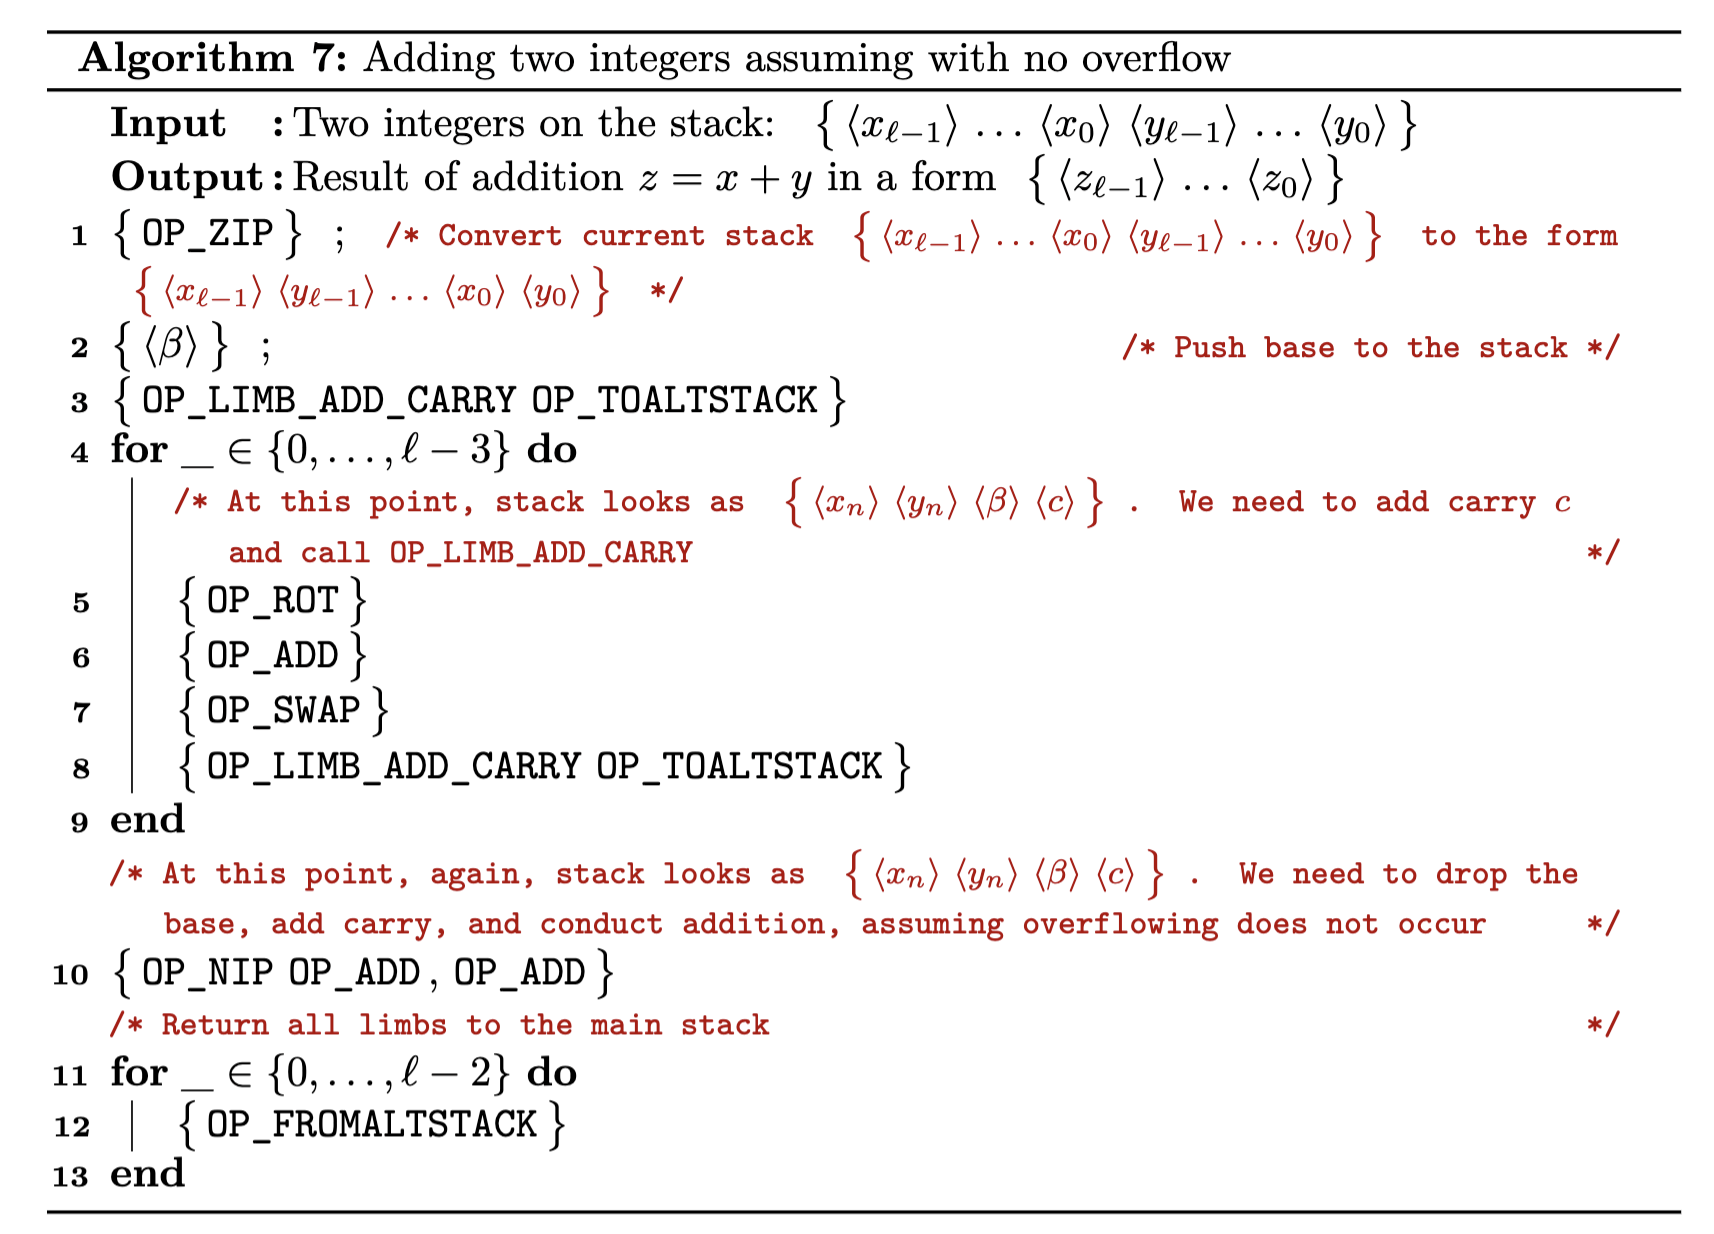
\includegraphics[width=\linewidth]{images/bigint_add.png}
        \end{figure}
    \end{frame}

    \begin{frame}[fragile]{BigInt Multiplication}
        \begin{block}{Problem}
            Given two 254-bit integers $x$ and $y$, find 508-bit $z := x \times y$.\pause
        \end{block}

        \small
        \begin{algorithm}[H]
          \caption{Double-and-add method for integer multiplication}\label{alg:double_and_add}
          \Input{$x,y$ --- two integers being multiplied}
          \Output{Result of the multiplication $x \times y$}
          
          Decompose $y$ to the binary form: $(y_0,y_1,\dots,y_{N-1})_2$
          
          $r \gets 0$
          
          $t \gets x$
          
          \For{$i \in \{0,\dots,N-1\}$}{
              \If{$y_i = 1$}{
                  $r \gets r + t$
              }
          
              $t \gets 2 \times t$
          }
          
          \Return{Integer $r$}
          
        \end{algorithm}
    \end{frame}

    \begin{frame}{Problem}
        \textbf{Problem:} If the cost of addition in $\mathsf{A}$ and of
        doubling is $\mathsf{D}$, the total algorithm's cost is
        $N\mathsf{A}+N\mathsf{D}$.\pause
        \begin{definition}
            The \textbf{$w$-width} form of a scalar $k \in \mathbb{Z}_{\geq 0}$
            is the representation:
            \begin{equation*}
                k = \sum_{i=0}^{L-1}k_i \times 2^{wi}, \quad 0 \leq k_i < 2^w,
            \end{equation*}
            where the decomposition length is $L = \lceil N/w \rceil$.\pause
        \end{definition}
        Using multiplication in such form, we will reduce the complexity down to:
        \begin{equation*}
            [2^{w-1}\mathsf{A}+2^{w-1}\mathsf{D}] + \left[\frac{N}{w}\mathsf{A}+N\mathsf{D}\right]
        \end{equation*}
    \end{frame}

    \begin{frame}{$w$-width BigInt Multiplication}
        \begin{algorithm}[H]
          \caption{Double-and-add method for integer multiplication}\label{alg:double_and_add}
          \Input{$x,y$ --- two integers being multiplied}
          \Output{Result of the multiplication $x \times y$}
          
          Decompose $y$ to the $w$-width form: $(y_0,y_1,\dots,y_{L-1})_w$

          Precompute $\{0x, 1x, 2x, \dots, (2^w-1)x\}$. Denote $\mathcal{T}[j]=jx$.
          
          $q \gets 0$
          
          \For{$i \in \{L-1,\dots,0\}$}{
              \For{$\_ \in \{1,\dots,w\}$}{
                 $q \gets 2q$
              }
              
              $q \gets q + \mathcal{T}[y_i]$
          }
          
          \Return{Integer $q$}
          
        \end{algorithm}
    \end{frame}

    \begin{frame}{Further Optimization}
        However, which value of $w$ to choose? In our research, we optimized 
        the cost function:
        \begin{equation*}
            C(w) = 2^{w-1}(C_A+C_D) + \frac{NC_A}{w} + NC_D\pause
        \end{equation*}
        \begin{itemize}
            \item $2^{w-1}(C_A+C_D)$ --- lookup table initialization cost.\pause
            \item $NC_A/w + NC_D$ --- cost of operations in the main loop.\pause
        \end{itemize}

        \begin{theorem}
            Optimal value is given by $\widehat{w}^22^{\widehat{w}} = \frac{2N}{\log 2} \cdot \frac{C_A}{C_A+C_D}$        
        \end{theorem}

        For BN254, we have $N=254$, $\widehat{w}=4$, so we need
        $72\mathsf{A}+262\mathsf{D}$ operations instead of
        $254\mathsf{A}+254\mathsf{D}$.
    \end{frame}

    \begin{frame}{What is left to optimize}
        How to prevent the overflowing when multiplying two $N$-bit integers
        $x,y$ and getting an $2N$-bit integer $z$?\pause

        \textcolor{blue!70!black}{\textbf{Naive approach:}} Extend $x,y$ to $2N$
        bit and conduct the algorithm as usual.\pause

        \textcolor{green!50!black}{\textbf{Better approach:}} Extend number of bits 
        of $x$ and $y$ gradually throughout the loop. 
    \end{frame}

    \begin{frame}{Results}
        \begin{figure}
            \centering
            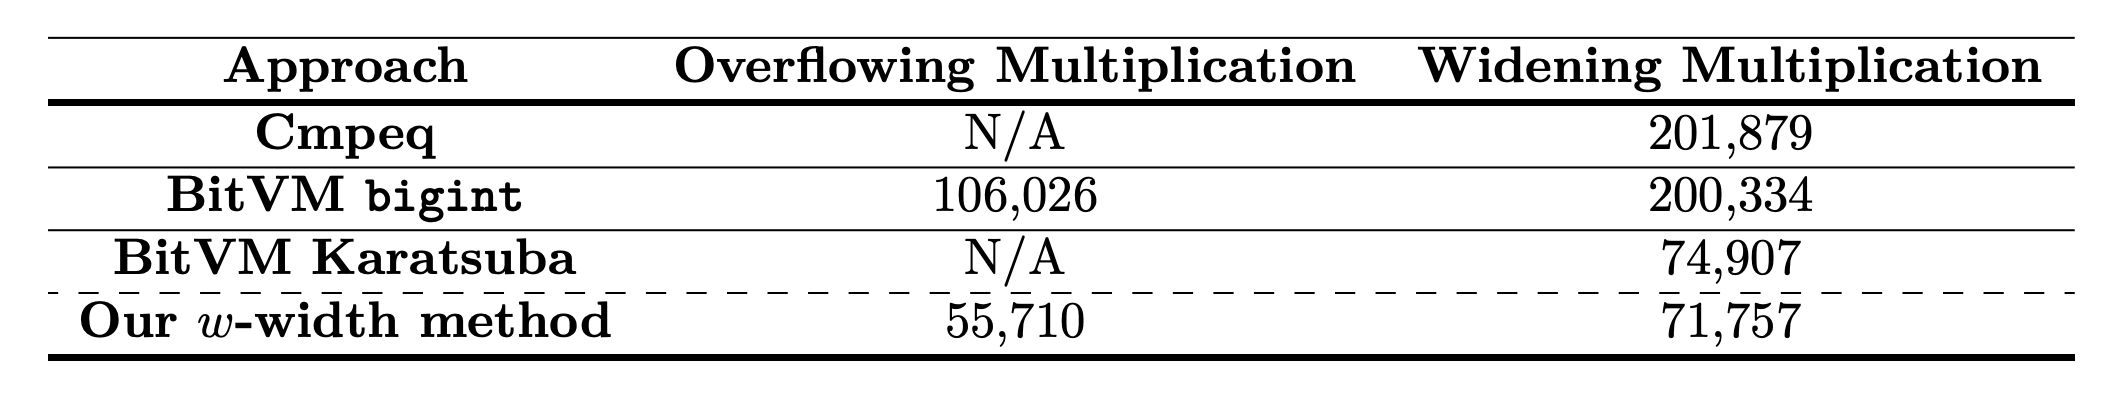
\includegraphics[width=\linewidth]{images/results.png}
        \end{figure}
        \begin{itemize}
            \item Besides better results in terms of OPCODEs \#, this 
            method allows to optimize MSM (batch multiplication). 
            \item As a result, our implementation is included in the BitVM codebase 
            and the total Groth16 script size is reduced $2\times$.
        \end{itemize}
    \end{frame}

    \begin{frame}[plain, standout]
        \centering
        \LARGE
        \textbf{Thank you for your attention} \\
        
        \vspace{0.2cm} \Huge \ding{170} \large \\
        
        \vspace{1cm}
  
        \href{https://distributedlab.com/}{\raisebox{-.1em}{\hspace{.025em}\faIcon{globe}}\hspace{.325em}distributedlab.com} \\
  
        \href{https://github.com/distributed-lab/bitcoin-window-mul}{\raisebox{-.1em}{\hspace{.025em}\faIcon{github}}\hspace{.325em}github.com/distributed-lab/bitcoin-window-mul}
    \end{frame}
\end{document}